\documentclass[12pt,a4paper]{report}

\usepackage[utf8]{inputenc}
\usepackage[T1]{fontenc}
\usepackage[english]{babel}
\usepackage[top=1cm,bottom=2cm,left=1cm,right=1cm]{geometry}
%\usepackage{url}
%\usepackage{fancyhdr}
\usepackage{sectsty}
\usepackage{wrapfig}
\usepackage{titlesec}
\usepackage{setspace}
\usepackage{graphicx}
\usepackage{lmodern}
\usepackage{url}
\usepackage{amsmath}
\usepackage{amssymb}
\usepackage{mathrsfs}
\usepackage{fancyhdr}
\usepackage{gensymb}
\usepackage{enumerate}
\usepackage{caption}
\usepackage{hyperref} % Créer des liens et des signets 
\usepackage[cc]{titlepic}
\usepackage{listing}

\title{
\rule{15cm}{1pt} \\
\Large {\bfseries Sensation and percetion} \\
\Large {\bfseries Assignement1}\\
\rule{15cm}{1pt}}
\author{Sami Sellami}

\titlepic{
\includegraphics[width=15cm]{Innopolis_image.png}} 
\date{\today}

\begin{document}
\pagenumbering{arabic}
\setcounter{page}{1}
\setcounter{secnumdepth}{1}
	
\fontfamily{ptm}\selectfont

\maketitle

\titlelabel{\thetitle)\quad}
\titlespacing{\chapter}{0cm}{0cm}{0cm}
\titlespacing{\section}{0.2cm}{0cm}{0cm}

THE SOURCE CODE IN GOOGLE COLABORATORY CAN BE FOUND IN THE LINK 
\href{https://colab.research.google.com/drive/1ftF9_4nVgUtGdKd0OFuLRP90zY1X1Ok4}{SourceCode}  

\textit{NB:the datasets must be uploaded in csv format}
\subsection{TASK 1: Case 4 Confidence interval and linear regression}
\subsection{Calculating the confidence intervel:}

We have a set of data points x and y representing the x-acceleration of the human CoM (Center of mass)as a function of time during the walking :

\begin{center}
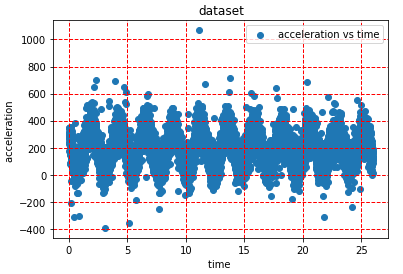
\includegraphics[width=10cm]{Capture1.png}
\captionof{figure}{Acceleration in respect of time}
\end{center}

We calculate the mean and standard deviation of t and x:

$$ \overline{t}= \frac{1}{N}\sum_{i=0}^N x_i= 12.99 \quad \sigma_t = \frac{1}{N} \sum_{i=0}^N (x_i - \overline{x})^2=7.50  $$
$$ \overline{x}= \frac{1}{N}\sum_{i=0}^N y_i= 197.85 \quad \sigma_x = \frac{1}{N} \sum_{i=0}^N (y_i - \overline{y})^2=126.55  $$

Now we have to remvove the outliers in the dataset, we use the instruction:
\begin{verbatim}
data= data[data.y<3*sd_y]
\end{verbatim}

and we obtain the following graph:
\begin{center}
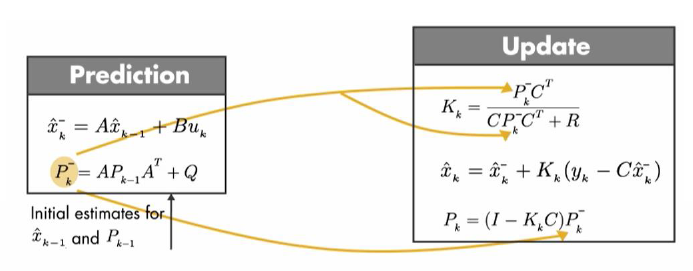
\includegraphics[width=10cm]{Capture2.png}
\captionof{figure}{Acceleration in respect of time after outliers elimination}
\end{center}

Now we will compute the confidence interval; $\quad \alpha = 1 - CL = 1-0.95 = 0.05$

The standard error is : $ \sigma_{\overline{x}} = \frac{\sigma_x}{\sqrt{N}}= 1.628 $

The z value for a confidence level corresponding to $CL=95$ is calculated like this:
 $$ P(0.95 + 0.05/2)= P(0.975) $$  
The z value for probability 0.9750 is 1.96 (using the standard normal table) 
The margin of error would be then: $ ME= z*\sigma_{\overline{x}}= 3.1932 $

And finally we can write the expression of the confidence interval :
$$CI = [\overline{x}- ME, \overline{x} + ME] = [194.661, 201.045]$$
It represent the interval in which the mean value of acceleration will be in 95 per cent of the time (the experiments)
 
\subsection{Performing the linear regression:}  
The graph of the data shows that the response follow a sinusoide in respect of time thus the true output can be written like this $$y(t)= A + B_0 \cos (\omega t+ \phi) = A + B \cos (\omega t) + C \sin(\omega t)$$ 
So for N observation we can write in matrix form:

$$ \left(\begin{array}{ccc} y(1)  \\ y(2)  \\ ... \\ y(n) \end{array}\right)
= \left(\begin{array}{ccc} 1 & \cos (\omega t(1)) & \sin(\omega t(1)) \\ 1 & \cos (\omega t(2)) & \sin(\omega t(2))  \\ ... & ...& ...\\ 1 & \cos (\omega t(N)) & \sin(\omega t(N)) \end{array}\right) 
\left(\begin{array}{ccc} A \\ B  \\ C \end{array}\right) + \left(\begin{array}{ccc} \epsilon_1 \\ \epsilon_2  \\ ... \\ \epsilon_N \end{array}\right)$$
In the form: $ Y= X \beta + \epsilon $ , and by minimizing the sum of squared erros we can find an estimate of the parameters:
$$ \beta = {(X^T X)}^{-1} X^T Y $$
But first we have to estimate the period of our signal; for that we perform the Fourrier transform of our data and we plot the corresponding power spectral density:

\begin{center}
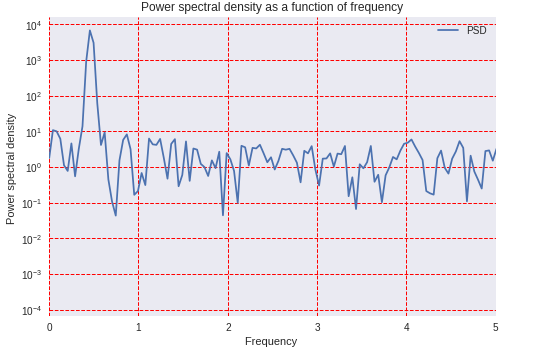
\includegraphics[width=10cm]{Capture3_bis.png}
\captionof{figure}{Power spectral density as a function of frequency}
\end{center}

From the graph we can see that the power spectral density has a pick at f= 0.43 Hz, which correspond to $\quad T=2.27  \quad \implies \omega = 2 \pi/T = 2.75 $

Now we can estimate the parameter $\beta$ using the formula shown above (see the code source in the link)and we obtain: 
$$\beta = \left(\begin{array}{ccc} 185.926 \\ 101.021  \\ -40.583 \end{array}\right)$$
The corresponding graph of the linear regression is as follows: 	
\begin{center}
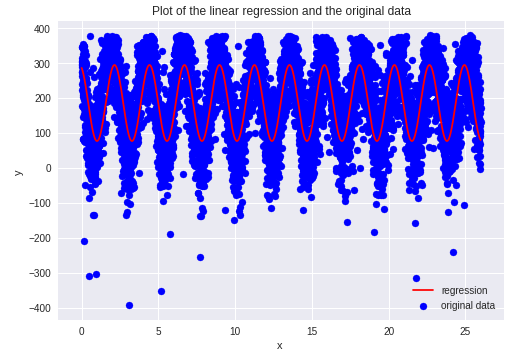
\includegraphics[width=10cm]{Capture3.png}
\captionof{figure}{Linear regression and dataset}
\end{center}

\subsection*{TASK 2 Case 17: RANSAC}
We have a set of data set in 3D as shown in the graph below: 
\begin{center}
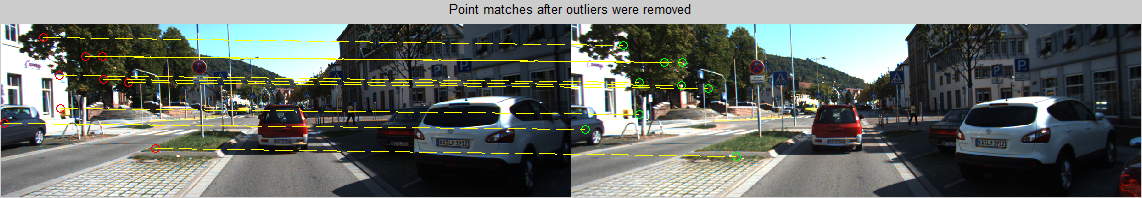
\includegraphics[width=7cm]{Capture4.png}
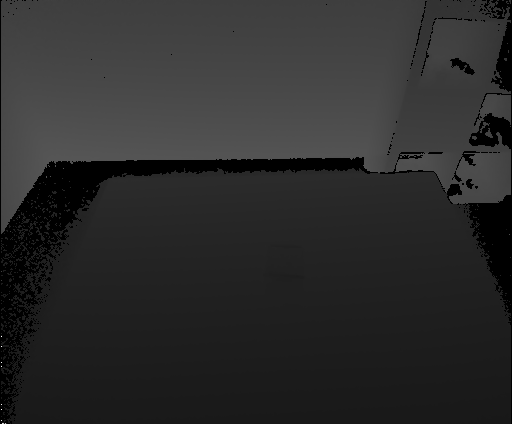
\includegraphics[width=7cm]{Capture5.png}
\captionof{figure}{Dataset in 3D }
\end{center}

After rotating the graph we clearly see that the dataset represent a plane in 3D and since we need 4 parameters to define a plane (model), the minimal sample set $ n = 4$ 

The number of iterations is calculated with the formula : 
$$  k=\frac{\log(1- P(success))}{\log(1- \omega^n)} $$
With a \quad $P(success)= 99$ \quad and\quad $ \omega  = 0.6$ \quad we obtain:\quad $ k = 18.9243 =18 $ 

Then we implement a function that estimate the parameters of the plane that best fits the datas using RANSAC algorithm:
\begin{verbatim}
def RANSAC(data2, k, threshold, d):  
  iteration=0
  while (iteration<k):
    r=[0, 0, 0]
    m_inlier=1.0*np.array([[0, 0, 0],[0, 0, 0], [0, 0, 0]])
    
    #we randomly select three points in the dataset
    for i in range(3): 
      r[i]= np.random.choice(range(99))
      m_inlier[i]=data2.iloc[r[i]]

    parameters=[0, 0, 0]
    parameters= plan(m_inlier[0, :], m_inlier[1, :], m_inlier[2, :])
    j=0
    i=0    
    n=np.array([parameters[0],parameters[1], parameters[2]])
    inlier=1.0*np.array([0, 0, 0])

    for i in range(99):
      #we verify if the distance between the plane and the point is less the threshold
      if(abs(parameters[0]*data2.x[i]+parameters[1]*data2.y[i]+parameters[2]*data2.z[i])/np.linalg.norm(n)<threshold):
        #np.concatenate((inlier, np.array(data2.iloc[1])), axis=1)    
        j=j+1
    
    if j>d:
      best_parameters=parameters
      d=j
    iteration=iteration+1
  return best_parameters
\end{verbatim}
By using the algorithm with a value of threshold equal to $t=3*standarddeviation =3* 0.68= 2.048 $, We find the parameters of the plane that best fits our dataset $\beta= \left[\begin{array}{cccc} a &b &c & d\end{array}\right]=\left[\begin{array}{cccc} -2.92 &-5.84 & -26.29 & -14.61\end{array}\right]$

And finally we can plot the plane obtained along with our dataset:

\begin{center}

\includegraphics[width=10cm]{Capture6.png}
\captionof{figure}{Dataset and regression plane in 3D }
\end{center}



\end{document}	
